\documentclass[10pt,a4paper]{report}
\usepackage[utf8]{inputenc}
\usepackage[russian]{babel}
\usepackage{amsmath}
\usepackage{amsfonts}
\usepackage{amssymb}
\usepackage{graphicx}
\renewcommand{\thesection}{\arabic{section}}
\setcounter{totalnumber}{10}
\setcounter{topnumber}{10}
\setcounter{bottomnumber}{10}
\renewcommand{\topfraction}{1}
\renewcommand{\textfraction}{0}
\author{Климов Сергей}
\title{Лабораторная работа №2.\\
	Утилита nmap}
\begin{document}
\maketitle
\tableofcontents
\pagebreak
	
\section{Цель работы}
Изучение принципов работы утилиты nmap.
\section{Описание окружения}
		Для проведения лабораторной работы было подготовлено две виртуальные машины, объединенные в общую сеть. Первая виртуальная машина (Metasploitable2), которая намеренно содержит ряд уязвимостей - целевая ВМ. Вторая виртуальная машина (Kali Linux) необходима для сканирования и поска уязвимостей на целевой ВМ.
		
		Целевая ВМ с ОС Metasploitable2 имеет адрес 169.254.120.103, ВМ Kali Linux имеет адрес 169.254.120.101.
		
		Конфигурация целевой ВМ:
		\begin{verbatim}  
        root@metasploitable:~$ ifconfig                                                
		eth0      Link encap:Ethernet  HWaddr 08:00:27:70:24:f3  
        inet addr:169.254.120.103  Bcast:169.254.255.255  Mask:255.255.0.0
        inet6 addr: fe80::a00:27ff:fe70:24f3/64 Scope:Link
        UP BROADCAST RUNNING MULTICAST  MTU:1500  Metric:1
        RX packets:11515 errors:0 dropped:0 overruns:0 frame:0
        TX packets:2319 errors:0 dropped:0 overruns:0 carrier:0
        collisions:0 txqueuelen:1000 
        RX bytes:1119307 (1.0 MB)  TX bytes:230624 (225.2 KB)
        Base address:0xd010 Memory:f0000000-f0020000 
		\end{verbatim}
		
		Конфигурация ВМ Kali Linux:
		\begin{verbatim}
		root@kali:~# ifconfig
		eth1: flags=4163<UP,BROADCAST,RUNNING,MULTICAST>  mtu 1500
        inet 169.254.120.101  netmask 255.255.0.0  broadcast 169.254.255.255
        inet6 fe80::a00:27ff:fe11:e70a  prefixlen 64  scopeid 0x20<link>
        ether 08:00:27:11:e7:0a  txqueuelen 1000  (Ethernet)
        RX packets 8532  bytes 838582 (818.9 KiB)
        RX errors 0  dropped 0  overruns 0  frame 0
        TX packets 253  bytes 20495 (20.0 KiB)
        TX errors 0  dropped 0 overruns 0  carrier 0  collisions 0
		\end{verbatim}


		Проверим доступность целевой ВМ при помощи утилиты ping:
		\begin{verbatim}
		root@kali:~# ping 169.254.120.103
		PING 169.254.120.103 (169.254.120.103) 56(84) bytes of data.
		64 bytes from 169.254.120.103: icmp_seq=1 ttl=64 time=0.554 ms
		64 bytes from 169.254.120.103: icmp_seq=2 ttl=64 time=0.756 ms
		64 bytes from 169.254.120.103: icmp_seq=3 ttl=64 time=0.697 ms
		64 bytes from 169.254.120.103: icmp_seq=4 ttl=64 time=0.740 ms
		^C
		--- 169.254.120.103 ping statistics ---
		4 packets transmitted, 4 received, 0% packet loss, time 3000ms
		rtt min/avg/max/mdev = 0.554/0.686/0.756/0.085 ms

		\end{verbatim}
		Как видно из результатов, целевая ВМ доступна в сети.

\section{Ход работы}		
		
	Дальнейшие действия будут выполняться с использованием утилиты nmap.
	\subsection{Поиск активных хостов}
	Для поиска активных хостов воспользуемся ключем -sP. Данный флаг указывает, что нужно искать сервера и устройства подключенные к сети и работающие в данный момент. В качестве параметра зададим нашу подсеть: 169.254.120.0/24.		
		Результат сканирования подсети на наличие активных хостов:
		\begin{verbatim}
		root@kali:~# nmap -sP 169.254.120.0/24

		Starting Nmap 7.01 ( https://nmap.org ) at 2016-04-03 05:24 EDT
		mass_dns: warning: Unable to determine any DNS servers. Reverse DNS 			is 	disabled. Try using --system-dns or specify valid servers with 				--dns-servers
		Nmap scan report for 169.254.120.2
		Host is up (0.0017s latency).
		MAC Address: 0A:00:27:00:00:15 (Unknown)
		Nmap scan report for 169.254.120.100
		Host is up (0.00089s latency).
		MAC Address: 08:00:27:8C:08:58 (Oracle VirtualBox virtual NIC)
		Nmap scan report for 169.254.120.103
		Host is up (0.0011s latency).
		MAC Address: 08:00:27:70:24:F3 (Oracle VirtualBox virtual NIC)
		Nmap scan report for 169.254.120.101
		Host is up.
		Nmap done: 256 IP addresses (4 hosts up) scanned in 1.82 seconds
		\end{verbatim}
		
		В результате сканирования, утилита нашла 4 активных хоста. Среди них видим наши виртуальные машины с адресами 169.254.120.101 и 169.254.120.103. 
		
	\subsection{Определение открытых портов целевой ВМ}
		Для сканирования портов хоста, утилите nmap необходимо передать адрес хоста, например:
		\begin{verbatim}
root@kali:~# nmap 169.254.120.103

Starting Nmap 7.01 ( https://nmap.org ) at 2016-04-03 05:38 EDT
mass_dns: warning: Unable to determine any DNS servers. Reverse DNS is disabled. Try using --system-dns or specify valid servers with --dns-servers
Nmap scan report for 169.254.120.103
Host is up (0.00067s latency).
Not shown: 977 closed ports
PORT     STATE SERVICE
21/tcp   open  ftp
22/tcp   open  ssh
23/tcp   open  telnet
25/tcp   open  smtp
53/tcp   open  domain
80/tcp   open  http
111/tcp  open  rpcbind
139/tcp  open  netbios-ssn
445/tcp  open  microsoft-ds
512/tcp  open  exec
513/tcp  open  login
514/tcp  open  shell
1099/tcp open  rmiregistry
1524/tcp open  ingreslock
2049/tcp open  nfs
2121/tcp open  ccproxy-ftp
3306/tcp open  mysql
5432/tcp open  postgresql
5900/tcp open  vnc
6000/tcp open  X11
6667/tcp open  irc
8009/tcp open  ajp13
8180/tcp open  unknown
MAC Address: 08:00:27:70:24:F3 (Oracle VirtualBox virtual NIC)

Nmap done: 1 IP address (1 host up) scanned in 0.23 seconds
		\end{verbatim}
		
		Как видно из вывода, на целевой ВМ открыто множество портов, например, 21 - ftp, 22 - ssh, 23 - telnet, 80 - http, а так же ряд других портов.
	\subsection{Определение версий сервисов}
	
	Для определения версий сервисов воспользуемся ключем -sV и передадим адрес целевой ВМ в качестве аргумента.
		\begin{verbatim}
		root@kali:~# nmap -sV 169.254.120.103

Starting Nmap 7.01 ( https://nmap.org ) at 2016-04-03 05:43 EDT
mass_dns: warning: Unable to determine any DNS servers. Reverse DNS is disabled. Try using --system-dns or specify valid servers with --dns-servers
Nmap scan report for 169.254.120.103
Host is up (0.00092s latency).
Not shown: 977 closed ports
PORT     STATE SERVICE     VERSION
21/tcp   open  ftp         vsftpd 2.3.4
22/tcp   open  ssh         OpenSSH 4.7p1 Debian 8ubuntu1 (protocol 2.0)
23/tcp   open  telnet      Linux telnetd
25/tcp   open  smtp        Postfix smtpd
53/tcp   open  domain      ISC BIND 9.4.2
80/tcp   open  http        Apache httpd 2.2.8 ((Ubuntu) DAV/2)
111/tcp  open  rpcbind     2 (RPC #100000)
139/tcp  open  netbios-ssn Samba smbd 3.X (workgroup: WORKGROUP)
445/tcp  open  netbios-ssn Samba smbd 3.X (workgroup: WORKGROUP)
512/tcp  open  tcpwrapped
513/tcp  open  tcpwrapped
514/tcp  open  tcpwrapped
1099/tcp open  rmiregistry GNU Classpath grmiregistry
1524/tcp open  tcpwrapped
2049/tcp open  nfs         2-4 (RPC #100003)
2121/tcp open  ftp         ProFTPD 1.3.1
3306/tcp open  mysql       MySQL 5.0.51a-3ubuntu5
5432/tcp open  postgresql  PostgreSQL DB 8.3.0 - 8.3.7
5900/tcp open  vnc         VNC (protocol 3.3)
6000/tcp open  X11         (access denied)
6667/tcp open  irc         Unreal ircd
8009/tcp open  ajp13       Apache Jserv (Protocol v1.3)
8180/tcp open  http        Apache Tomcat/Coyote JSP engine 1.1
MAC Address: 08:00:27:70:24:F3 (Oracle VirtualBox virtual NIC)
Service Info: Hosts:  metasploitable.localdomain, localhost, irc.Metasploitable.LAN; OSs: Unix, Linux; CPE: cpe:/o:linux:linux_kernel

Service detection performed. Please report any incorrect results at https://nmap.org/submit/ .
Nmap done: 1 IP address (1 host up) scanned in 16.63 seconds

		\end{verbatim}	
		
		В результате видим, что утилита nmap вывела нам версии сервисов, запущенных на целевой ВМ.
		
	\subsection{Исследование служебных файлов nmap-services, nmap-os-db, nmap-service-probes}
		Служебные файлы для утилиты nmap по умолчанию располагаются в директории "/usr/share/nmap".
		\subsubsection{Файл nmap-services}
		Файл nmap-services является реестром, где хранятся названия портов (служб на них работающих), их номера и названия протовкола. https://nmap.org/book/nmap-services.html
Файл имеет структуру таблицы со следующими столбцами: имя\_сервиса, номер\_порта/название\_протокола, частота, комментарии.
			Часть данного файла:
			\begin{verbatim}
ftp-data	20/udp	0.001878	# File Transfer [Default Data]
ftp	21/sctp	0.000000	# File Transfer [Control]
ftp	21/tcp	0.197667	# File Transfer [Control]
ftp	21/udp	0.004844	# File Transfer [Control]
ssh	22/sctp	0.000000	# Secure Shell Login
ssh	22/tcp	0.182286	# Secure Shell Login
ssh	22/udp	0.003905	# Secure Shell Login
telnet	23/tcp	0.221265
			\end{verbatim}
			
			Для "свободных" номеров портов, файл так же содержит записи, но они не несут никакой полезной информации, что ожидаемо, так как на этих портах запускаются пользовательские сервисы, и они не закреплены ни за одним приложением.
			\begin{verbatim}
unknown	249/tcp	0.000050
unknown	250/tcp	0.000138
unknown	251/tcp	0.000125
unknown	252/tcp	0.000088
			\end{verbatim}
			
			
		\subsubsection{Файл nmap-os-db}
			Данный файл содержит сигнатуры ответов различных операционных систем при сканировании утилитой nmap. Это необходимо для того, что бы узнать какая операционная система находится на данном хосте. Пример файла nmap-os-db:
			\begin{verbatim}
root@kali:~# head /usr/share/nmap/nmap-os-db -n92906 | tail -n10
# Arris Interactive, L.L.C. MODEL: TM402G SW_REV: 6.1.77D.D11PLUS
# bizhub C203
Fingerprint VxWorks
Class Wind River | VxWorks || general purpose
CPE cpe:/o:windriver:vxworks auto
SEQ(SP=FE-10A%GCD=1-6%ISR=FC-10E%TI=I%CI=I%II=I%SS=S%TS=8)
OPS(O1=M5B4NW0NNT11%O2=M5B4NW0NNT11%O3=M5B4NW0NNT11%O4=M5B4NW0NNT11%O5=M5B4NW0NNT11%O6=M5B4NNT11)
WIN(W1=4000%W2=4000%W3=4000%W4=4000%W5=4000%W6=4000)
ECN(R=Y%DF=Y%T=3B-45%TG=40%W=4000%O=M5B4NW0%CC=N%Q=)
T1(R=Y%DF=Y%T=3B-45%TG=40%S=O%A=S+%F=AS%RD=0%Q=)
			\end{verbatim}

		\subsubsection{Файл nmap-service-probes}
			Данный файл содержит сигнатуры для определения сервисов, прослушивающих тот или иной порт. Как правило, это относится к известным службам, например SMTP - почтовый сервис. Данные о сервисах задаются при помощи нескольких директив:
			\begin{itemize}
				\item Exclude <port specification>
				\item Probe <protocol> <probename> <probestring>
				\item match <service> <pattern> [<versioninfo>]
			\end{itemize}
	\subsection{Добавление собственной сигнатуры в файл nmap-service-probes}
		Для того, что бы добавить собственную сигнатуру, создадим небольшой сервер, который мы будем идентифицировать при помощи утилиты nmap. Код сервера представлен ниже:
		\begin{verbatim}
#include <sys/socket.h> 
#include <netinet/in.h> 
#include <arpa/inet.h> 
#include <stdio.h> 
#include <stdlib.h> 
#include <string.h> 
#include <unistd.h> 
#define DEF_PORT 19931 
int main(int argc, char** argv) { 
	char str[100];
	char *sendStr="sergServ 0.3";
	struct sockaddr_in listenerInfo; 
	listenerInfo.sin_family = AF_INET; 
	listenerInfo.sin_port = htons(DEF_PORT); 
	listenerInfo.sin_addr.s_addr = htonl(INADDR_ANY); 
	int listener = socket(AF_INET,SOCK_STREAM,0); 
	if(listener < 0) { 
		perror("Can't create socket to listen: "); 
		exit(1); 
	} 
	int res = bind(listener,(struct sockaddr *) &listenerInfo,sizeof(listenerInfo)); 
	if(res < 0) { 
		perror("Can't bind socket"); 
		exit(1); 
	} 
	res = listen(listener,5); 
	if(res) { 
		perror("Erro while listening:"); 
		exit(1); 
	}
	int client = accept(listener,NULL,NULL);
	while(1) {
		bzero( str, 100);
		recv(client,str, 100, 0); 
		printf("Message from client - %s",str);
		send(client, sendStr, (int)strlen(sendStr), 0);
	}
	return 0; 
}
		\end{verbatim}
		Сервер работатет на порте 19931. Серверу отправляется строка 'qqSerg' и он отвечает строкой со своим именем и версией: 'sergServ v0.3'.
		
		Для определения данного сервера в файл nmap-service-probes были добавлены следующие строки:
		\begin{verbatim}
			#####Test sergServ
			Probe TCP sergServ q|qqSerg|
			rarity 1
			ports 19931
			match sergServ m|sergServ (...+?)| v/$1/
		\end{verbatim}
		
		Запустим на испытуемой виртуальной машине данный сервер и попробуем определить его при помощи утилиты nmap:
		\begin{verbatim}
root@kali:~# nmap 169.254.120.101 -p 19931 -sV

Starting Nmap 7.01 ( https://nmap.org ) at 2016-04-03 22:49 MSK
mass_dns: warning: Unable to determine any DNS servers. Reverse DNS is disabled. Try using --system-dns or specify valid servers with --dns-servers
Nmap scan report for 169.254.120.101
Host is up (0.000067s latency).
PORT      STATE SERVICE  VERSION
19931/tcp open  sergServ 0.3

Service detection performed. Please report any incorrect results at https://nmap.org/submit/ .
Nmap done: 1 IP address (1 host up) scanned in 6.91 seconds

		\end{verbatim}
		Как видно из вывода, утилита корректно определила наш сервер.
		
	\subsection{Сохранение вывода утилиты nmap в формате XML}
		Для сохранения вывода утилиты nmap в формате  XML необходимо при 
		запуске указать ключ '-oX':
		\begin{verbatim}
			nmap -oX - 169.254.120.103 > out.xml
		\end{verbatim}
		В результате запуска, утилитой nmap будут просканированы все порты хоста с адресом 169.254.120.103, и вывод будет сохранен в формате 
		XML. Содержимое файла out.xml:
		\begin{verbatim}
			<?xml version="1.0" encoding="UTF-8"?>
<!DOCTYPE nmaprun>
<?xml-stylesheet href="file:///usr/bin/../share/nmap/nmap.xsl" type="text/xsl"?>
<!-- Nmap 7.01 scan initiated Sun Apr  3 07:42:02 2016 as: nmap -oX - 169.254.120.103 -->
<nmaprun scanner="nmap" args="nmap -oX - 169.254.120.103" start="1459683722" startstr="Sun Apr  3 07:42:02 2016" version="7.01" xmloutputversion="1.04">
<scaninfo type="syn" protocol="tcp" numservices="1000" services="1,3-4,6-7,9,13,17,19-26,30,32-33,37,42-43,49,53,70,79-85,88-90,99-100,106,109-111,113,119,125,135,139,143-144,146,161,163,179,199,211-212,222,254-256,259,264,280,301,306,311,340,366,389,406-407,416-417,425,427,443-445,458,464-465,481,497,500,512-515,524,541,543-545,548,554-555,563,587,593,616-617,625,631,636,646,648,666-668,683,687,691,700,705,711,714,720,722,726,749,765,777,783,787,800-801,808,843,873,880,888,898,900-903,911-912,981,987,990,992-993,995,999-1002,1007,1009-1011,1021-1100,1102,1104-1108,1110-1114,1117,1119,1121-1124,1126,1130-1132,1137-1138,1141,1145,1147-1149,1151-1152,1154,1163-1166,1169,1174-1175,1183,1185-1187,1192,1198-1199,1201,1213,1216-1218,1233-1234,1236,1244,1247-1248,1259,1271-1272,1277,1287,1296,1300-1301,1309-1311,1322,1328,1334,1352,1417,1433-1434,1443,1455,1461,1494,1500-1501,1503,1521,1524,1533,1556,1580,1583,1594,1600,1641,1658,1666,1687-1688,1700,1717-1721,1723,1755,1761,1782-1783,1801,1805,1812,1839-1840,1862-1864,1875,1900,1914,1935,1947,1971-1972,1974,1984,1998-2010,2013,2020-2022,2030,2033-2035,2038,2040-2043,2045-2049,2065,2068,2099-2100,2103,2105-2107,2111,2119,2121,2126,2135,2144,2160-2161,2170,2179,2190-2191,2196,2200,2222,2251,2260,2288,2301,2323,2366,2381-2383,2393-2394,2399,2401,2492,2500,2522,2525,2557,2601-2602,2604-2605,2607-2608,2638,2701-2702,2710,2717-2718,2725,2800,2809,2811,2869,2875,2909-2910,2920,2967-2968,2998,3000-3001,3003,3005-3007,3011,3013,3017,3030-3031,3052,3071,3077,3128,3168,3211,3221,3260-3261,3268-3269,3283,3300-3301,3306,3322-3325,3333,3351,3367,3369-3372,3389-3390,3404,3476,3493,3517,3527,3546,3551,3580,3659,3689-3690,3703,3737,3766,3784,3800-3801,3809,3814,3826-3828,3851,3869,3871,3878,3880,3889,3905,3914,3918,3920,3945,3971,3986,3995,3998,4000-4006,4045,4111,4125-4126,4129,4224,4242,4279,4321,4343,4443-4446,4449,4550,4567,4662,4848,4899-4900,4998,5000-5004,5009,5030,5033,5050-5051,5054,5060-5061,5080,5087,5100-5102,5120,5190,5200,5214,5221-5222,5225-5226,5269,5280,5298,5357,5405,5414,5431-5432,5440,5500,5510,5544,5550,5555,5560,5566,5631,5633,5666,5678-5679,5718,5730,5800-5802,5810-5811,5815,5822,5825,5850,5859,5862,5877,5900-5904,5906-5907,5910-5911,5915,5922,5925,5950,5952,5959-5963,5987-5989,5998-6007,6009,6025,6059,6100-6101,6106,6112,6123,6129,6156,6346,6389,6502,6510,6543,6547,6565-6567,6580,6646,6666-6669,6689,6692,6699,6779,6788-6789,6792,6839,6881,6901,6969,7000-7002,7004,7007,7019,7025,7070,7100,7103,7106,7200-7201,7402,7435,7443,7496,7512,7625,7627,7676,7741,7777-7778,7800,7911,7920-7921,7937-7938,7999-8002,8007-8011,8021-8022,8031,8042,8045,8080-8090,8093,8099-8100,8180-8181,8192-8194,8200,8222,8254,8290-8292,8300,8333,8383,8400,8402,8443,8500,8600,8649,8651-8652,8654,8701,8800,8873,8888,8899,8994,9000-9003,9009-9011,9040,9050,9071,9080-9081,9090-9091,9099-9103,9110-9111,9200,9207,9220,9290,9415,9418,9485,9500,9502-9503,9535,9575,9593-9595,9618,9666,9876-9878,9898,9900,9917,9929,9943-9944,9968,9998-10004,10009-10010,10012,10024-10025,10082,10180,10215,10243,10566,10616-10617,10621,10626,10628-10629,10778,11110-11111,11967,12000,12174,12265,12345,13456,13722,13782-13783,14000,14238,14441-14442,15000,15002-15004,15660,15742,16000-16001,16012,16016,16018,16080,16113,16992-16993,17877,17988,18040,18101,18988,19101,19283,19315,19350,19780,19801,19842,20000,20005,20031,20221-20222,20828,21571,22939,23502,24444,24800,25734-25735,26214,27000,27352-27353,27355-27356,27715,28201,30000,30718,30951,31038,31337,32768-32785,33354,33899,34571-34573,35500,38292,40193,40911,41511,42510,44176,44442-44443,44501,45100,48080,49152-49161,49163,49165,49167,49175-49176,49400,49999-50003,50006,50300,50389,50500,50636,50800,51103,51493,52673,52822,52848,52869,54045,54328,55055-55056,55555,55600,56737-56738,57294,57797,58080,60020,60443,61532,61900,62078,63331,64623,64680,65000,65129,65389"/>
<verbose level="0"/>
<debugging level="0"/>
<host starttime="1459683722" endtime="1459683723"><status state="up" reason="arp-response" reason_ttl="0"/>
<address addr="169.254.120.103" addrtype="ipv4"/>
<address addr="08:00:27:70:24:F3" addrtype="mac" vendor="Oracle VirtualBox virtual NIC"/>
<hostnames>
</hostnames>
<ports><extraports state="closed" count="977">
<extrareasons reason="resets" count="977"/>
</extraports>
<port protocol="tcp" portid="21"><state state="open" reason="syn-ack" reason_ttl="64"/><service name="ftp" method="table" conf="3"/></port>
<port protocol="tcp" portid="22"><state state="open" reason="syn-ack" reason_ttl="64"/><service name="ssh" method="table" conf="3"/></port>
<port protocol="tcp" portid="23"><state state="open" reason="syn-ack" reason_ttl="64"/><service name="telnet" method="table" conf="3"/></port>
<port protocol="tcp" portid="25"><state state="open" reason="syn-ack" reason_ttl="64"/><service name="smtp" method="table" conf="3"/></port>
<port protocol="tcp" portid="53"><state state="open" reason="syn-ack" reason_ttl="64"/><service name="domain" method="table" conf="3"/></port>
<port protocol="tcp" portid="80"><state state="open" reason="syn-ack" reason_ttl="64"/><service name="http" method="table" conf="3"/></port>
<port protocol="tcp" portid="111"><state state="open" reason="syn-ack" reason_ttl="64"/><service name="rpcbind" method="table" conf="3"/></port>
<port protocol="tcp" portid="139"><state state="open" reason="syn-ack" reason_ttl="64"/><service name="netbios-ssn" method="table" conf="3"/></port>
<port protocol="tcp" portid="445"><state state="open" reason="syn-ack" reason_ttl="64"/><service name="microsoft-ds" method="table" conf="3"/></port>
<port protocol="tcp" portid="512"><state state="open" reason="syn-ack" reason_ttl="64"/><service name="exec" method="table" conf="3"/></port>
<port protocol="tcp" portid="513"><state state="open" reason="syn-ack" reason_ttl="64"/><service name="login" method="table" conf="3"/></port>
<port protocol="tcp" portid="514"><state state="open" reason="syn-ack" reason_ttl="64"/><service name="shell" method="table" conf="3"/></port>
<port protocol="tcp" portid="1099"><state state="open" reason="syn-ack" reason_ttl="64"/><service name="rmiregistry" method="table" conf="3"/></port>
<port protocol="tcp" portid="1524"><state state="open" reason="syn-ack" reason_ttl="64"/><service name="ingreslock" method="table" conf="3"/></port>
<port protocol="tcp" portid="2049"><state state="open" reason="syn-ack" reason_ttl="64"/><service name="nfs" method="table" conf="3"/></port>
<port protocol="tcp" portid="2121"><state state="open" reason="syn-ack" reason_ttl="64"/><service name="ccproxy-ftp" method="table" conf="3"/></port>
<port protocol="tcp" portid="3306"><state state="open" reason="syn-ack" reason_ttl="64"/><service name="mysql" method="table" conf="3"/></port>
<port protocol="tcp" portid="5432"><state state="open" reason="syn-ack" reason_ttl="64"/><service name="postgresql" method="table" conf="3"/></port>
<port protocol="tcp" portid="5900"><state state="open" reason="syn-ack" reason_ttl="64"/><service name="vnc" method="table" conf="3"/></port>
<port protocol="tcp" portid="6000"><state state="open" reason="syn-ack" reason_ttl="64"/><service name="X11" method="table" conf="3"/></port>
<port protocol="tcp" portid="6667"><state state="open" reason="syn-ack" reason_ttl="64"/><service name="irc" method="table" conf="3"/></port>
<port protocol="tcp" portid="8009"><state state="open" reason="syn-ack" reason_ttl="64"/><service name="ajp13" method="table" conf="3"/></port>
<port protocol="tcp" portid="8180"><state state="open" reason="syn-ack" reason_ttl="64"/><service name="unknown" method="table" conf="3"/></port>
</ports>
<times srtt="284" rttvar="152" to="100000"/>
</host>
<runstats><finished time="1459683723" timestr="Sun Apr  3 07:42:03 2016" elapsed="0.27" summary="Nmap done at Sun Apr  3 07:42:03 2016; 1 IP address (1 host up) scanned in 0.27 seconds" exit="success"/><hosts up="1" down="0" total="1"/>
</runstats>
</nmaprun>

		\end{verbatim}
	\subsection{Исследование работы утилиты nmap при помощи wireshark}
	
	Запустим утилиту WireShark, затем просканируем целевую ВМ по адресу 169.254.120.103.
		\begin{verbatim}
		root@kali:~# nmap 169.254.120.103
		\end{verbatim}

Как показано на рисунке \ref{ris:image1}. Изначально nmap посылат на существующие порты TCP-пакеты с установленным флагом SYN, что означает установление соединения. Если при этом сканируемый порт отправляет ответ с установленными флагами [RST, ACK], значит соединение невозможно - порт закрыт.\\
Если после отправки TCP-пакета с флагом SYN сканируемый порт отправляет ответ также с установленным флагом SYN, это означает, что заданый порт открыт. Это таакже видно на рисунке \ref{ris:image1}.\\
\begin{figure}[ht]	\center{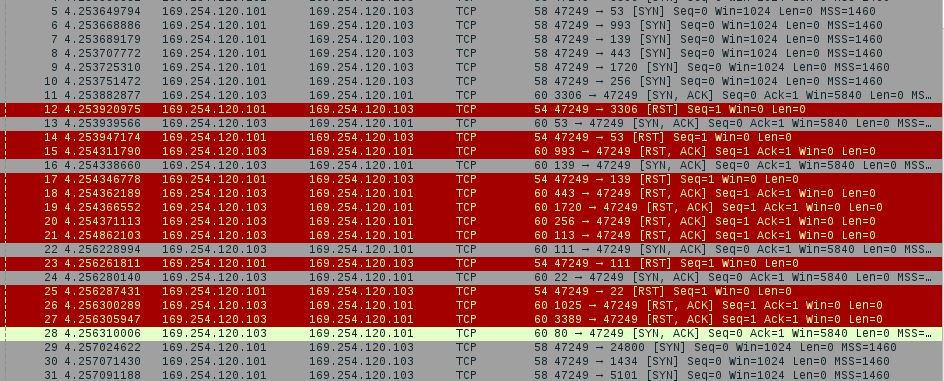
\includegraphics[width=1\linewidth]{images/1}}
\caption{Вывод утилиты WireShark.}\label{ris:image1}
\end{figure} \\		
		
		\subsection{Просканировать виртуальную машину Metasploitable2 используя db\_nmap из состава metasploit-framework}
		Перед началом сканировании необходимо включить postgresql и выполнить команду msfdb init для инициализации базы данных:
		\begin{verbatim}
root@kali:~# service postgresql start
root@kali:~# msfdb init
Creating database user 'msf'
Enter password for new role: 
Enter it again: 
Creating databases 'msf' and 'msf_test'
Creating configuration file in /usr/share/metasploit-framework/config/database.yml
Creating initial database schema
		\end{verbatim}
		После чего необходимо запустить msfconsole и можно использовать любую из команд, описанных выше, но вместо nmap можно использовать db\_map. Результаты работы будут записаны в базу данных, тем самым обеспечивая экономию времени при сканировании портов.
		\begin{verbatim}
root@kali:~# msfconsole
                                                  

  Metasploit Park, System Security Interface
  Version 4.0.5, Alpha E
  Ready...
  > access security
  access: PERMISSION DENIED.
  > access security grid
  access: PERMISSION DENIED.
  > access main security grid
  access: PERMISSION DENIED....and...
  YOU DIDN'T SAY THE MAGIC WORD!
  YOU DIDN'T SAY THE MAGIC WORD!
  YOU DIDN'T SAY THE MAGIC WORD!
  YOU DIDN'T SAY THE MAGIC WORD!
  YOU DIDN'T SAY THE MAGIC WORD!
  YOU DIDN'T SAY THE MAGIC WORD!
  YOU DIDN'T SAY THE MAGIC WORD!


Save 45% of your time on large engagements with Metasploit Pro
Learn more on http://rapid7.com/metasploit

       =[ metasploit v4.11.7-                             ]
+ -- --=[ 1518 exploits - 877 auxiliary - 259 post        ]
+ -- --=[ 437 payloads - 38 encoders - 8 nops             ]
+ -- --=[ Free Metasploit Pro trial: http://r-7.co/trymsp ]

msf > db_nmap 169.254.120.103
[*] Nmap: Starting Nmap 7.01 ( https://nmap.org ) at 2016-04-04 00:12 MSK
[*] Nmap: 'mass_dns: warning: Unable to determine any DNS servers. Reverse DNS is disabled. Try using --system-dns or specify valid servers with --dns-servers'
[*] Nmap: Nmap scan report for 169.254.120.103
[*] Nmap: Host is up (0.0010s latency).
[*] Nmap: Not shown: 977 closed ports
[*] Nmap: PORT     STATE SERVICE
[*] Nmap: 21/tcp   open  ftp
[*] Nmap: 22/tcp   open  ssh
[*] Nmap: 23/tcp   open  telnet
[*] Nmap: 25/tcp   open  smtp
[*] Nmap: 53/tcp   open  domain
[*] Nmap: 80/tcp   open  http
[*] Nmap: 111/tcp  open  rpcbind
[*] Nmap: 139/tcp  open  netbios-ssn
[*] Nmap: 445/tcp  open  microsoft-ds
[*] Nmap: 512/tcp  open  exec
[*] Nmap: 513/tcp  open  login
[*] Nmap: 514/tcp  open  shell
[*] Nmap: 1099/tcp open  rmiregistry
[*] Nmap: 1524/tcp open  ingreslock
[*] Nmap: 2049/tcp open  nfs
[*] Nmap: 2121/tcp open  ccproxy-ftp
[*] Nmap: 3306/tcp open  mysql
[*] Nmap: 5432/tcp open  postgresql
[*] Nmap: 5900/tcp open  vnc
[*] Nmap: 6000/tcp open  X11
[*] Nmap: 6667/tcp open  irc
[*] Nmap: 8009/tcp open  ajp13
[*] Nmap: 8180/tcp open  unknown
[*] Nmap: MAC Address: 08:00:27:70:24:F3 (Oracle VirtualBox virtual NIC)
[*] Nmap: Nmap done: 1 IP address (1 host up) scanned in 0.40 seconds

		\end{verbatim}
	\subsection{Описать работу пяти записей из файла nmap-service-probes}
	\begin{verbatim}	
	Probe UDP AndroMouse q|AMSNIFF|
	rarity 9
	ports 8888
	match AndroMouse m|^GOTBACK$|s p/AndroMouse Android remote mouse server/
	\end{verbatim}	
	
Директива Probe указывает на то, какое сообщение необходимо отправить для индентификации сервиса. В данном случае, сервис - AndroMouse, используемый протокол - UDP, отправляется следующая строка:

\begin{verbatim}
AMSNIFF
\end{verbatim}

Строка с директивой rarity указывает частоту, с которой от сервиса можно ожидать возвращения корректных результатов. В данном случае - 9. \\
Директива ports указывает на порты, используемые данным сервисом. \\
Директива match необходима при распознавании сервиса на основе ответов на строку, отправленную предыдущей директивой Probe.

	\subsection{Описать работу скрипта из состава Nmap}

Рассмотрим скрипт imap-capabilities. Данный скрипт получает информацию об IMAP mail сервере и выводит список поддерживаемых команд из RFC 3501.
		Пример использования:
		\begin{verbatim}
			root@kali:~# nmap -script=imap-capabilities imap.yandex.ru

Starting Nmap 7.01 ( https://nmap.org ) at 2016-04-04 01:27 MSK
Nmap scan report for imap.yandex.ru (93.158.134.124)
Host is up (0.0023s latency).
Other addresses for imap.yandex.ru (not scanned): 213.180.193.124 213.180.204.124 77.88.21.124 87.250.251.124 2a02:6b8::124
Not shown: 998 filtered ports
PORT    STATE SERVICE
143/tcp open  imap
|_imap-capabilities: CHILDREN XLIST MOVEA0001 ID NAMESPACE IMAP4rev1 STARTTLS ENABLE LITERAL+ UNSELECT BINARY IDLE Completed UIDPLUS CAPABILITY OK LOGINDISABLED
993/tcp open  imaps
|_imap-capabilities: UIDPLUS AUTH=PLAIN CHILDREN CAPABILITY XLIST MOVEA0001 OK ID NAMESPACE IDLE IMAP4rev1 Completed ENABLE UNSELECT LITERAL+ BINARY

Nmap done: 1 IP address (1 host up) scanned in 5.87 seconds

		\end{verbatim}
		Код скрипта:
		\begin{verbatim}
		local imap = require "imap"
local shortport = require "shortport"
local stdnse = require "stdnse"
local table = require "table"

description = [[
Retrieves IMAP email server capabilities.

IMAP4rev1 capabilities are defined in RFC 3501. The CAPABILITY command
allows a client to ask a server what commands it supports and possibly
any site-specific policy.
]]

---
-- @output
-- 143/tcp open  imap
-- |_ imap-capabilities: LOGINDISABLED IDLE IMAP4 LITERAL+ STARTTLS NAMESPACE IMAP4rev1


author = "Brandon Enright"
license = "Same as Nmap--See https://nmap.org/book/man-legal.html"

categories = {"default", "safe"}


portrule = shortport.port_or_service({143, 993}, {"imap", "imaps"})

local function fail (err) return stdnse.format_output(false, err) end

action = function(host, port)
  local helper = imap.Helper:new(host, port)
  local status = helper:connect()
  if ( not(status) ) then return fail("Failed to connect to server") end

  local status, capa = helper:capabilities(host, port)
  if( not(status) ) then return fail("Failed to retrieve capabilities") end
  helper:close()

  if type(capa) == "table" then
    -- Convert the capabilities table into an array of strings.
    local capstrings = {}
    local cap, args
    for cap, args in pairs(capa) do
      table.insert(capstrings, cap)
    end
    return stdnse.strjoin(" ", capstrings)
  elseif type(capa) == "string" then
    stdnse.debug1("'%s' for %s", capa, host.ip)
    return
  else
    return "server doesn't support CAPABILITIES"
  end
end
		\end{verbatim}
		В данном скрипте проверяются два стандартных порта для подкючения к IMAP серверу - 143 и 993(ssl). Далее вызывается встпомогательная функция, которая запрашивает список поддерживаемых команд сервером, затем происходит перевод их в строку для вывода пользователю.
		
		\section{Выводы}
			В ходе данной лабораторной работы было произведено ознакомление с утилитой nmap. Был получен опят ее приенения для сканирования открытых портов и доступных хостов, а также для определения версий сервисов. Также были рассмотрены основные служебные файлы, которые используются для работы данной утилиты: файлы конфигураций и скрипты. Было рассмотрено расширение db\_map, которое позволяет сохранять результаты сканирования в базу данных, тем самым увеличивая скорость работы утилиты.
\end{document}